\section{实验原理}
\subsection{单周期改流水线原理}
实验三已完成图中单周期的部分,可以看到,流水线处理器的主要改动,是在每个执行阶段加入触发器,使得每个周期执行一个阶段,得到的结果送往下一个周期进行执行,同时下一条指令执行一个阶段,这样能够使指令各阶段并行执行,提升效率。 

\begin{figure}[htbp]
    \centering
    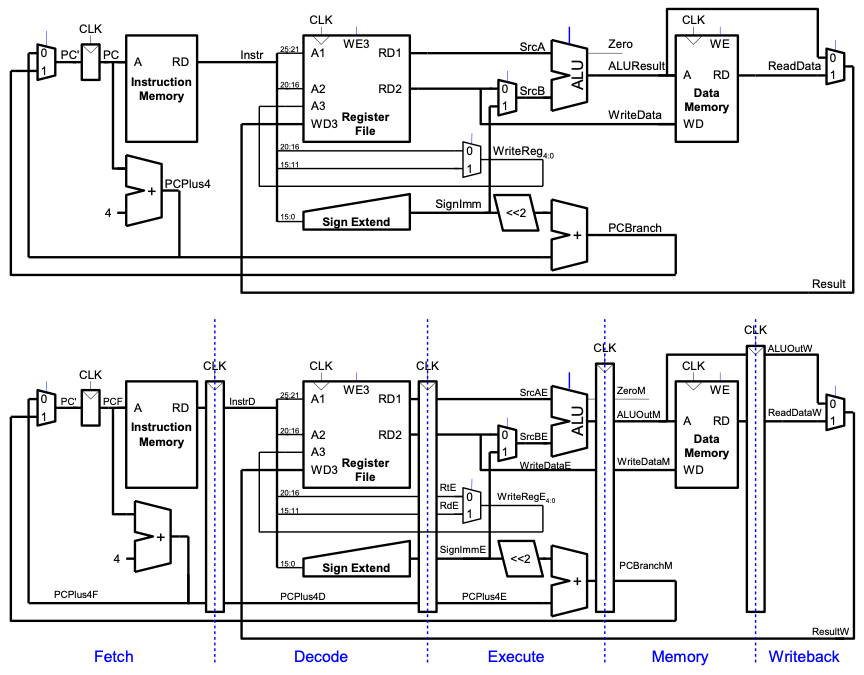
\includegraphics[width = 0.95\textwidth]{image/single_piped.png}
    \caption{单周期和流水线比较}
    \label{fig:section_2_0}
\end{figure}

可以看到,单周期中写寄存器堆的地址信号writereg需要延迟到writeback阶段与回写数据result一起写回寄存器堆:

\newpage
\begin{figure}[htbp]
    \centering
    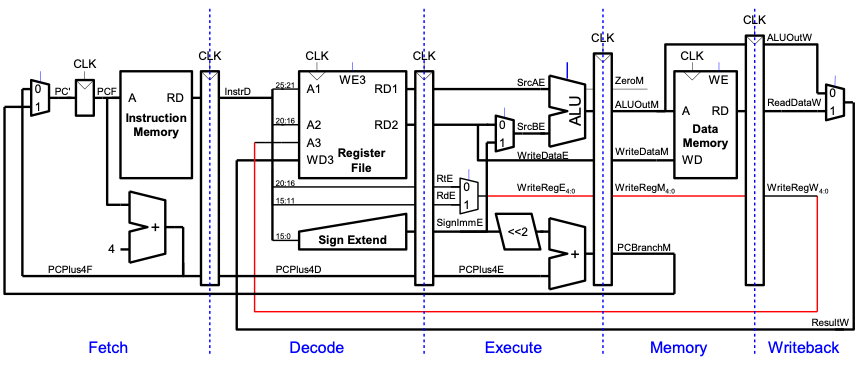
\includegraphics[width = 0.95\textwidth]{image/piped_writereg.png}
    \caption{修改writereg信号}
    \label{fig:section_2_1}
\end{figure}

在此基础上,datapath的基本通路已经形成,下面加入控制器部分。控制器部分与单周期相同,仍然由main decoder和alu decoder构成,但由于改为五级流水线后,每一个阶段所需要的控制信号仅为一部分,控制器产生信号的阶段为译码阶段,产生控制信号后,依次通过触发器传到下一阶段,若当前阶段需要的信号,则不需要继续传递到下一阶段:

\begin{figure}[htbp]
    \centering
    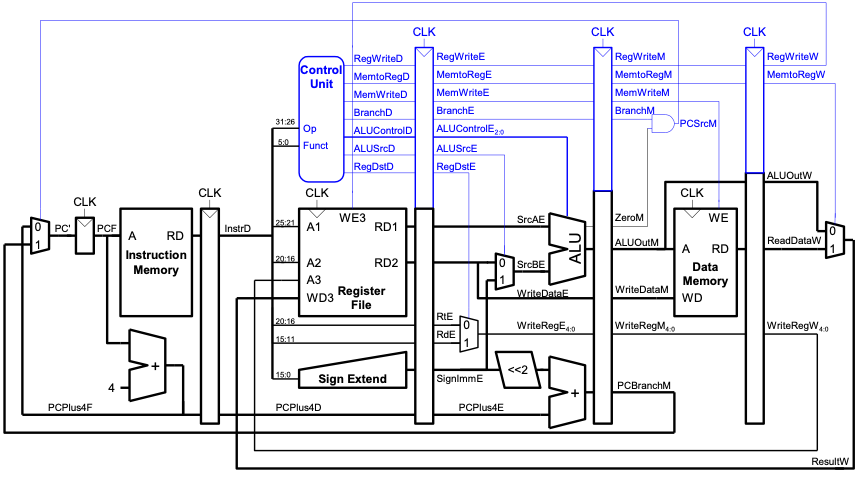
\includegraphics[width = 0.95\textwidth]{image/piped_with_controller.png}
    \caption{加入控制器的流水线示意图}
    \label{fig:section_2_2}
\end{figure}
\subsection{各类型触发器的实现}
实验三中已给出触发器flopr,作为PC使用,此外需要在其基础上实现下列触发器,:
\begin{itemize}
    \item flopr:带有reset的触发器
	\item floprc:带有reset与clear的触发器
	\item flopenrc:带有enable、reset与clear的触发器
\end{itemize}

flopr的写法如下:
\begin{lstlisting}[language=Verilog,label=lst:3_stage_pipeline,caption=flopr实现,numbers=left,xleftmargin=5em,xrightmargin=5em, aboveskip=2em]
module flopr #(parameter WIDTH = 8)(
	input wire clk, rst,
	input wire[WIDTH-1:0] d,
	output reg[WIDTH-1:0] q
    );

	always @(posedge clk,posedge rst) begin
		if(rst) begin
			q <= 0;
		end else begin 
			q <= d;
		end
	end
endmodule
\end{lstlisting}

floprc的写法如下:
\begin{lstlisting}[language=Verilog,caption=floprc实现,numbers=left,xleftmargin=5em,xrightmargin=5em, aboveskip=2em]
module floprc #(parameter WIDTH = 8)(
	input wire clk,rst,clear,
	input wire[WIDTH-1:0] d,
	output reg[WIDTH-1:0] q
    );

	always @(posedge clk,posedge rst) begin
		if(rst) begin
			q <= 0;
		end else if (clear)begin
			q <= 0;
		end else begin 
			q <= d;
		end
	end
endmodule
\end{lstlisting}


flopenrc的写法如下:
\begin{lstlisting}[language=Verilog,caption=flopenrc实现,numbers=left,xleftmargin=5em,xrightmargin=5em, aboveskip=2em]
module flopenrc #(parameter WIDTH = 8)(
	input wire clk,rst,en,clear,
	input wire[WIDTH-1:0] d,
	output reg[WIDTH-1:0] q
    );
	always @(posedge clk) begin
		if(rst) begin
			q <= 0;
		end else if(clear) begin
			q <= 0;
		end else if(en) begin
			/* code */
			q <= d;
		end
	end
endmodule
\end{lstlisting}


注意\textbf{\#(parameter WIDTH = 8)}的写法,这样写,在调用时可以指定宽度:

\begin{lstlisting}[language=Verilog,caption=带参数实例化,numbers=left,xleftmargin=5em,xrightmargin=4em, aboveskip=2em]
flopenrc #(32) r1M(clk,rst,~stallM,flushM,srcb2E,writedataM);
flopenrc #(32) r2M(clk,rst,~stallM,flushM,aluout2E,aluoutM);
flopenrc #(5)  r3M(clk,rst,~stallM,flushM,writereg2E,writeregM);
\end{lstlisting}

\subsection{冒险(hazard)的解决}
在流水线CPU中,并不是能够完全实现并行执行。在单周期中由于每条指令执行完毕才会执行下一条指令,并不会遇到冒险问题,而在流水线处理器中,由于当前指令可能取决于前一条指令的结果,但此时前一条指令并未执行到产生结果的阶段,这时候,就产生了冒险。
	
冒险分为:
\begin{enumerate}
    \item 数据冒险:寄存器中的值还未写回到寄存器堆中,下一条指令已经需要从寄存器堆中读取数据;
	\item 控制冒险:下一条要执行的指令还未确定,就按照PC自增顺序执行了本不该执行的指令(由分支指令引起)。
\end{enumerate}

\subsubsection{数据冒险}
\begin{figure}[htbp]
    \centering
    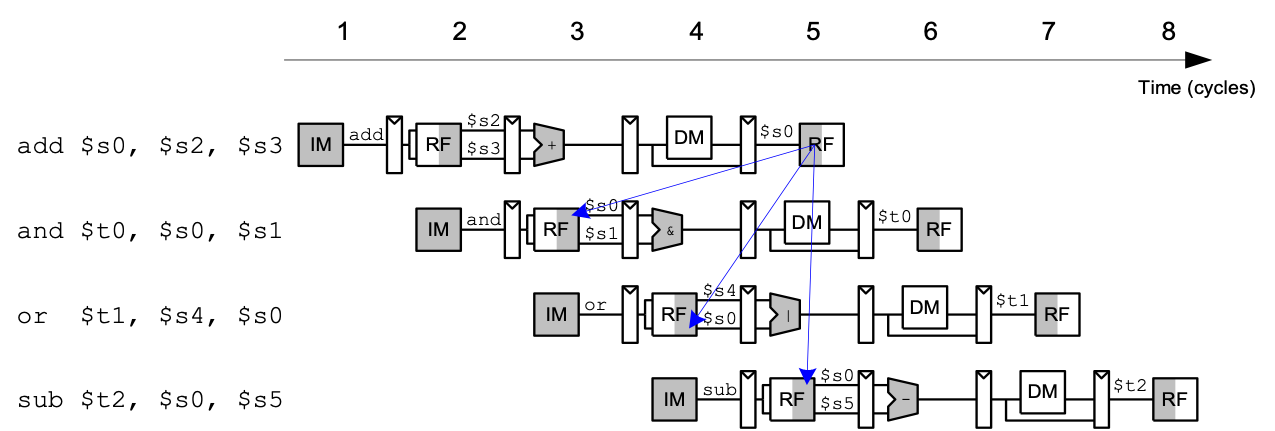
\includegraphics[width = 0.95\textwidth]{image/data_hazard.png}
    \caption{数据冒险示例}
    \label{fig:section_2_3}
\end{figure}
分析图~\ref{fig:section_2_3}中指令,and、or、sub指令均需要使用\$s0中的数据,然而add指令在回写阶段才能写入寄存器堆,此时后续三条指令均已经过或正在执行译码阶段,得到的结果均为错误值。
以上就是数据冒险的特点,数据冒险有以下解决方式:
\begin{enumerate}
    \item 在编译时插入空指令;
    \item 在编译时对指令执行顺序进行重排;
    \item 在执行时进行数据前推;
    \item 在执行时,暂停处理器当前阶段的执行,等待结果。
\end{enumerate}
由于我们未进行编译层的处理,需要在运行时(run time)进行解决,故采用3、4解决方案。

\subsubsection{数据前推}
\begin{figure}[htbp]
    \centering
    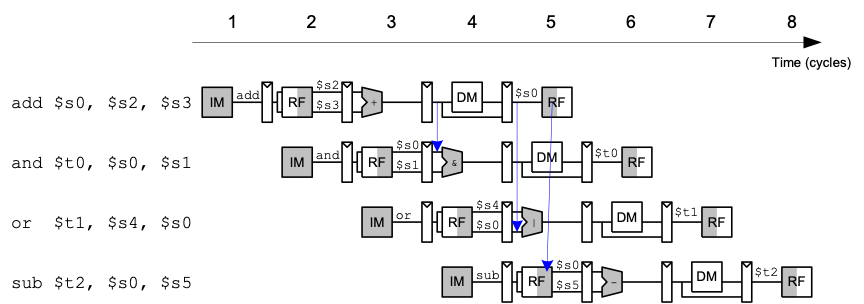
\includegraphics[width = 0.95\textwidth]{image/data_forward.png}
    \caption{数据前推示例}
    \label{fig:section_2_4}
\end{figure}

从图~\ref{fig:section_2_4}中可以看到,add指令的结果在execute阶段已经由ALU计算得到,此时可以将alu得到的结果直接推送到下一条指令的execute阶段,同理,后续所有的阶段均已有结果,可以向对应的阶段推送,而不需要等到回写后再进行读取,达到数据前推的目的。

数据前推的实现逻辑如下:
\begin{lstlisting}[language=Verilog,caption=数据前推的实现逻辑,numbers=left,xleftmargin=5em,xrightmargin=5em, aboveskip=2em]
if  ((rsE != 0) AND (rsE == WriteRegM) AND RegWriteM)     
	then 	
	    ForwardAE = 10
else if ((rsE != 0) AND (rsE == WriteRegW) AND RegWriteW) 
	then 	
	    ForwardAE = 01
else
    ForwardAE = 00

\end{lstlisting}
结合实现逻辑,观察下图。在execute阶段需要判断当前输入ALU的地址是否与其他指令在此时执行的阶段要写入寄存器堆的地址相同,如果相同,就需要将其他指令的结果直接通过多路选择器输入到ALU中。

此处需要:
\begin{enumerate}
    \item 增加rs,rt的地址传递到execute阶段,并与冒险模块连接;
    \item Memory阶段和writeback阶段要写入寄存堆的地址与冒险模块连接;
    \item Memory阶段和writeback阶段的寄存器堆写使能信号regwrite与冒险模块连接;
    \item 根据实现逻辑,将生成的forward信号输出,控制mux3选择器。
\end{enumerate}

数据通路结构如下:
\begin{figure}[htbp]
    \centering
    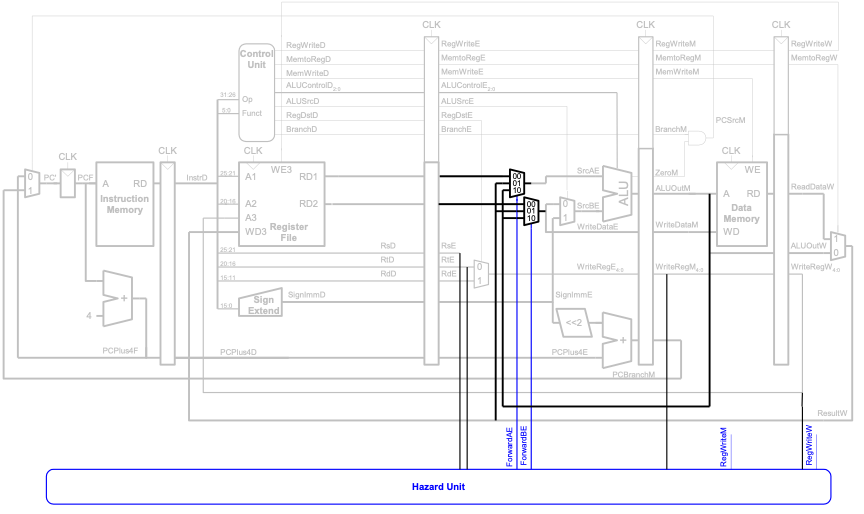
\includegraphics[width = 0.95\textwidth]{image/hazard.png}
    \caption{加入前推的数据通路结构}
    \label{fig:section_2_5}
\end{figure}

\subsubsection{流水线暂停}
\begin{figure}[htbp]
    \centering
    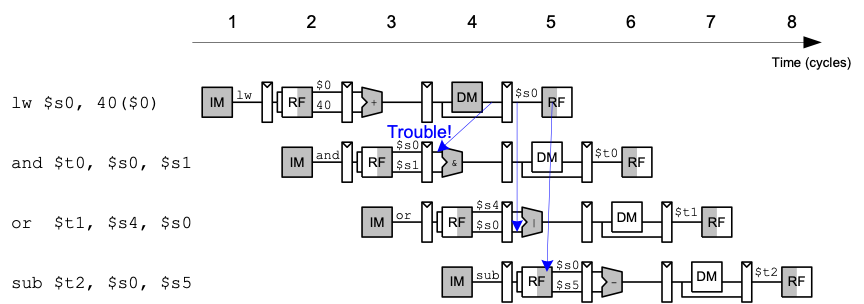
\includegraphics[width = 0.95\textwidth]{image/data_forward_failed.png}
    \caption{数据无法前推的情况}
    \label{fig:section_2_6}
\end{figure}

\begin{figure}[htbp]
    \centering
    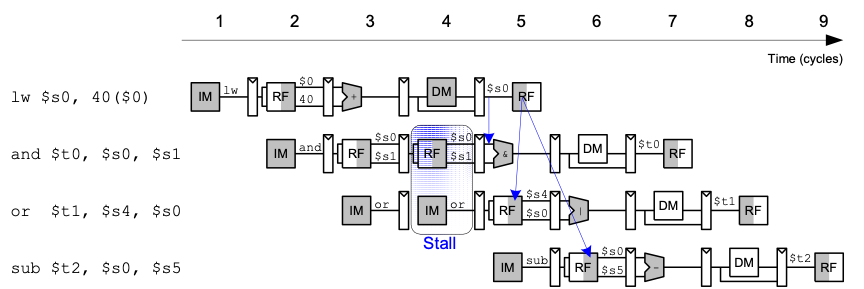
\includegraphics[width = 0.95\textwidth]{image/pipe_pause.png}
    \caption{流水线暂停示例}
    \label{fig:section_2_7}
\end{figure}

多数情况下,数据前推能解决很大一部分数据冒险的问题,然而在图中~\ref{fig:section_2_6},lw指令在memory阶段才能够从数据存储器读取数据,此时and指令已经完成ALU计算,无法进行数据前推。
	
如图~\ref{fig:section_2_7}在这种情况下,必须使流水线暂停,等待数据读取后,再前推到execute阶段。

流水线暂停的实现逻辑如下:
\begin{lstlisting}[language=Verilog,caption=流水线暂停的实现逻辑,numbers=left,xleftmargin=5em,xrightmargin=5em, aboveskip=2em]
lwstall = ((rsD==rtE) OR (rtD==rtE)) AND MemtoRegE
StallF = StallD = FlushE = lwstall
\end{lstlisting}

结合实现逻辑,需要完成下列功能:
\begin{enumerate}
    \item 判断decode阶段rs或rt的地址是否是lw指令要写入的地址;
    \item 设置PC、fetch->decode阶段触发器的暂停信号(触发器使能端disable);
    \item Decode->exexcute阶段触发器清除(避免后续阶段的执行,等待完成后方可继续执行后续阶段)。
\end{enumerate}

数据通路结构如下:
\begin{figure}[htbp]
    \centering
    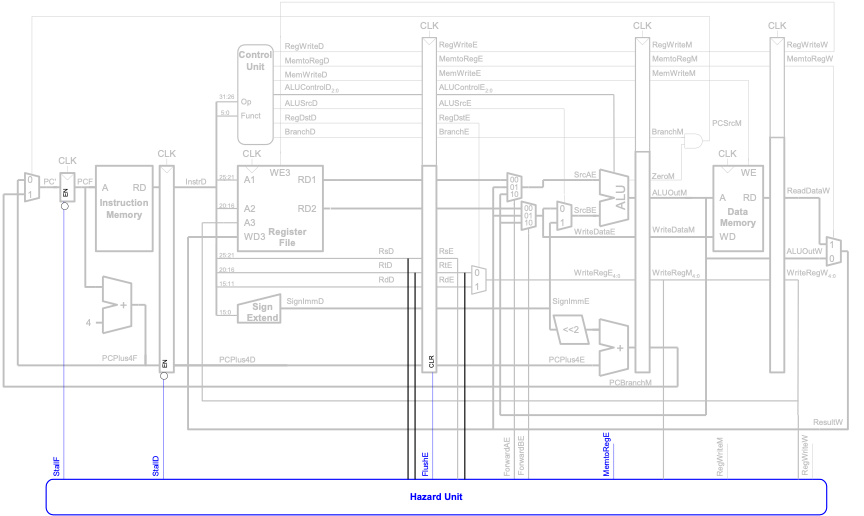
\includegraphics[width = 0.95\textwidth]{image/hazard_with_pause.png}
    \caption{加入暂停的数据通路结构}
    \label{fig:section_2_8}
\end{figure}

\newpage

\subsubsection{控制冒险}
控制冒险是分支指令引起的冒险。在五级流水线当中,分支指令在第4阶段才能够决定是否跳转;而此时,前三个阶段已经导致三条指令进入流水线开始执行,这时需要将这三条指令产生的影响全部清除。
\begin{figure}[htbp]
    \centering
    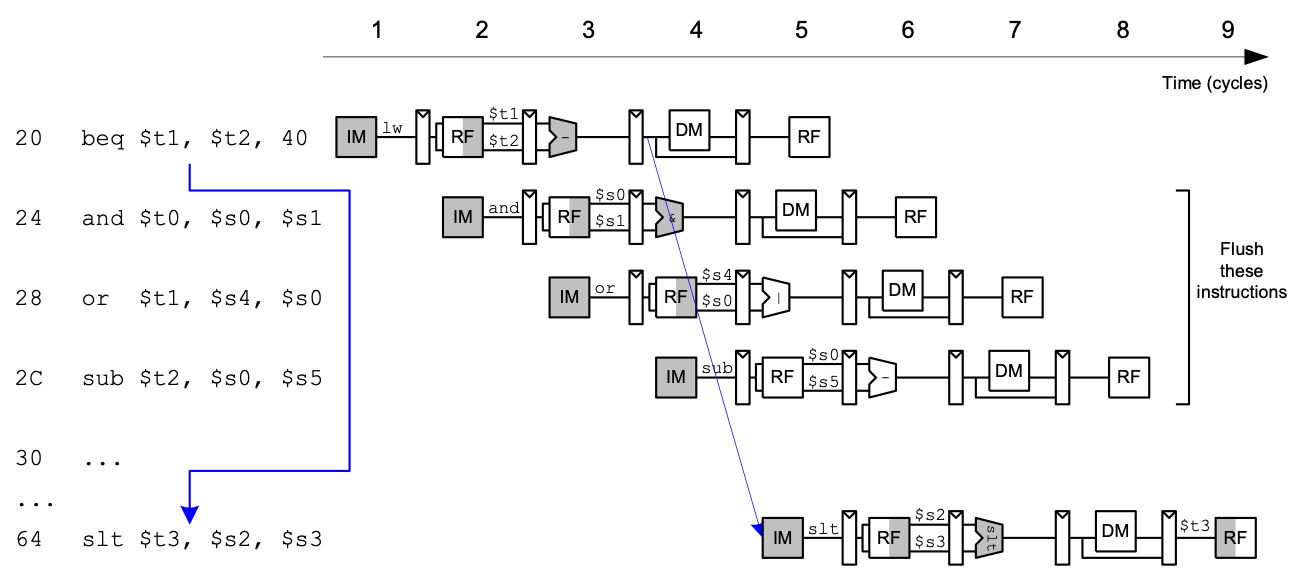
\includegraphics[width = 0.95\textwidth]{image/control_hazard.png}
    \caption{控制冒险示例}
    \label{fig:section_2_9}
\end{figure}

将分支指令的判断提前至decode阶段,此时能够减少两条指令的执行;
\begin{figure}[htbp]
    \centering
    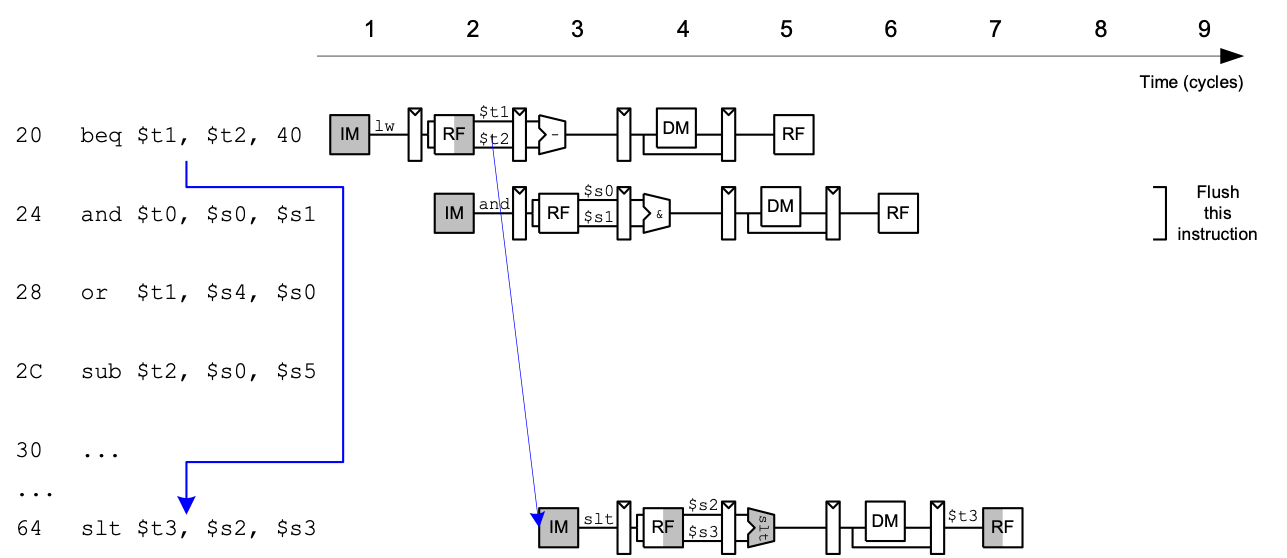
\includegraphics[width = 0.95\textwidth]{image/early_branch.png}
    \caption{提前判断分支}
    \label{fig:section_2_9}
\end{figure}

\newpage
在regfile输出后添加一个判断相等的模块,即可提前判断beq:
\begin{figure}[htbp]
    \centering
    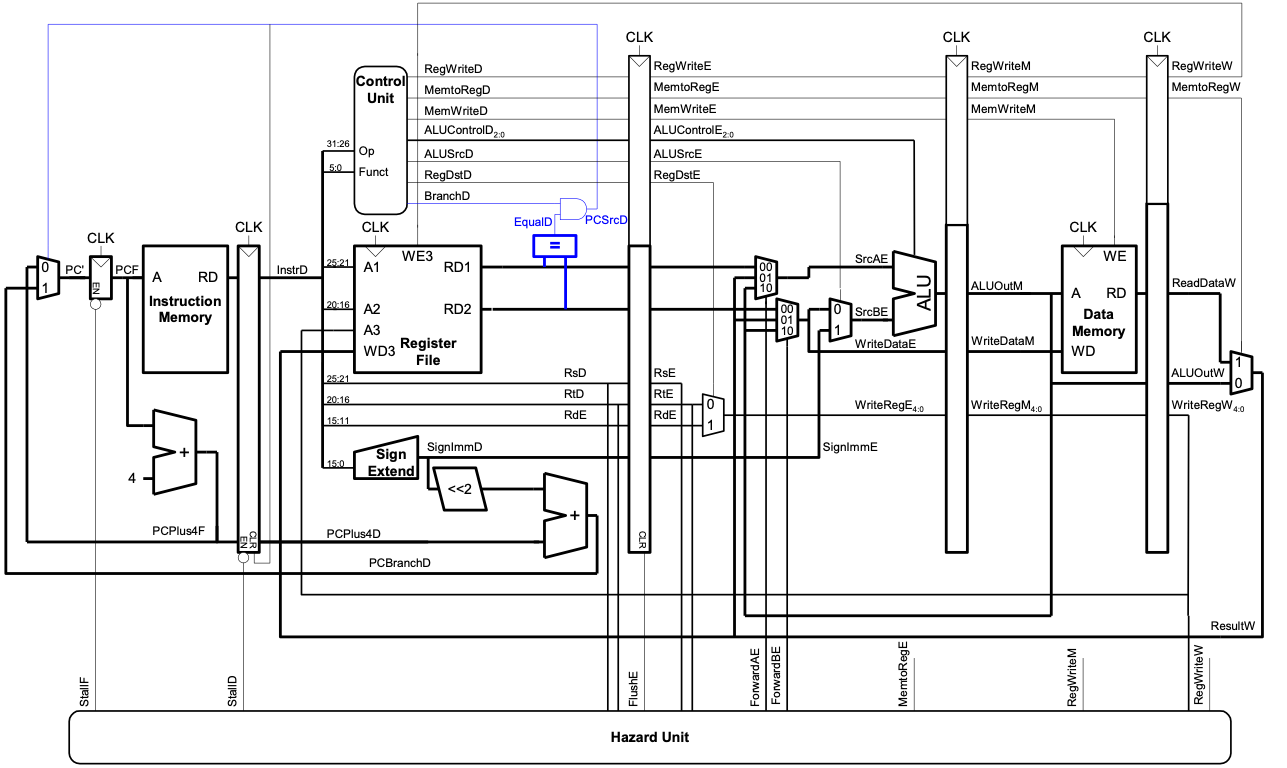
\includegraphics[width = 0.95\textwidth]{image/pre-condition.png}
    \caption{提前判断分支的实现}
    \label{fig:section_2_9}
\end{figure}

\newpage
此时又产生了数据冲突问题,需要增加数据前推和流水线暂停模块;

\begin{figure}[htbp]
    \centering
    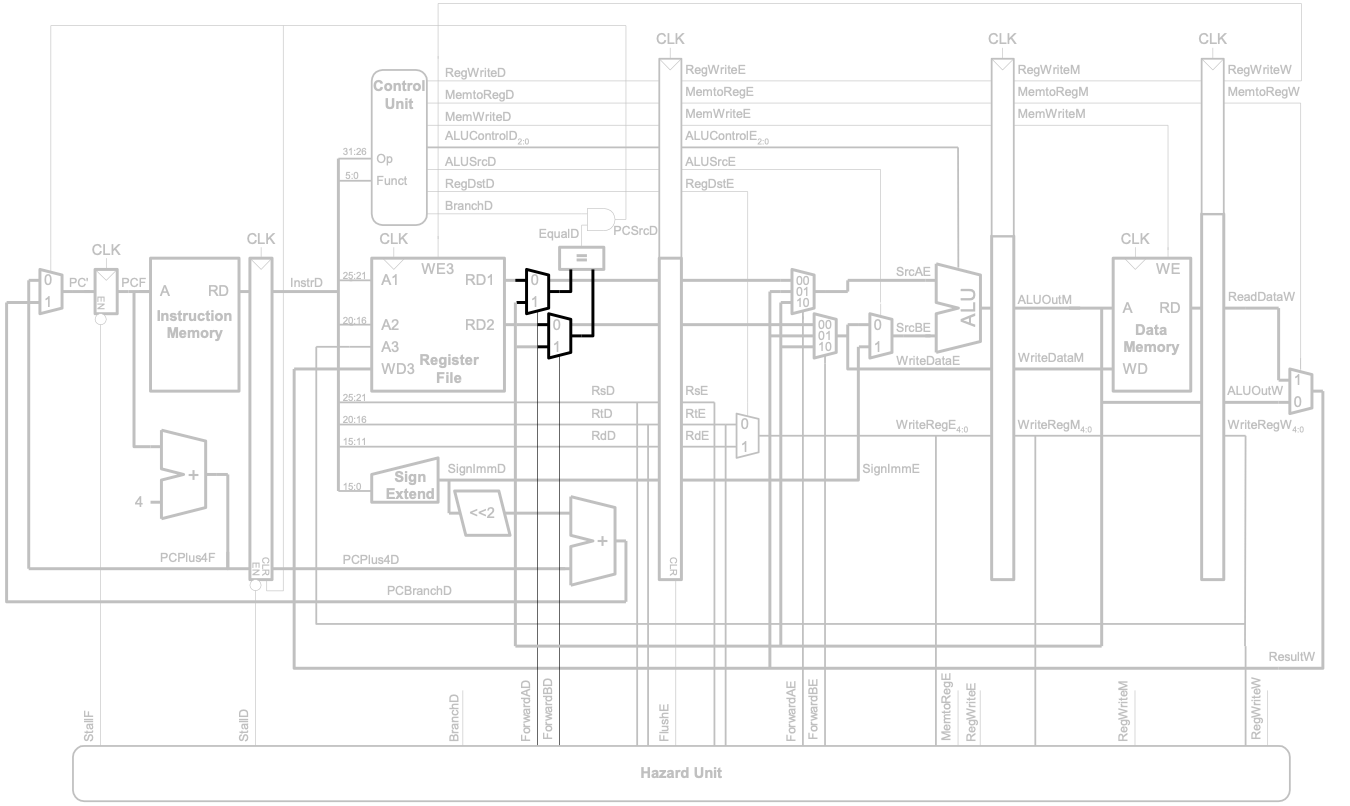
\includegraphics[width = 0.95\textwidth]{image/hazard_handle_control_hazard.png}
    \caption{解决控制冒险的数据通路}
    \label{fig:section_2_9}
\end{figure}

实现逻辑如下:
Forwarding logic:
\begin{lstlisting}[language=Verilog,caption=控制冒险前推的实现逻辑,numbers=left,xleftmargin=5em,xrightmargin=5em, aboveskip=2em]
	ForwardAD = (rsD !=0) AND (rsD == WriteRegM) AND RegWriteM
	ForwardBD = (rtD !=0) AND (rtD == WriteRegM) AND RegWriteM
\end{lstlisting}

Stalling logic:
\begin{lstlisting}[language=Verilog,caption=控制冒险暂停的实现逻辑,numbers=left,xleftmargin=5em,xrightmargin=5em, aboveskip=2em]
	branchstall = BranchD AND RegWriteE AND 
                   (WriteRegE == rsD OR WriteRegE == rtD) 
                 OR BranchD AND MemtoRegM AND 
                   (WriteRegM == rsD OR WriteRegM == rtD)
	StallF = StallD = FlushE = lwstall OR branchstall
\end{lstlisting}

